% Basic setup. Most papers should leave these options alone.
\documentclass[fleqn,usenatbib]{mnras}

%\hypersetup{draft}

\usepackage[T1]{fontenc}
\usepackage{ae,aecompl}

\usepackage{graphicx}	% Including figure files
\usepackage{amsmath}	% Advanced maths commands
\usepackage{color}

\usepackage{mathptmx}
\usepackage{txfonts}

% Macros
\newcommand{\blue}[1]{{\color{blue} #1}}
\newcommand{\kmsmpc}{\kms\;{\rm Mpc}^{-1}}
\newcommand{\rvir}{$r_{\rm vir}$}
\newcommand{\lya}{Ly$\alpha$}
\newcommand{\HI}{\ion{H}{i}}
\newcommand{\OHI}{\Omega_{\rm HI}}
\newcommand{\sHI}{\sigma_{\rm HI}}
\newcommand{\nhi}{N_{\rm HI}}
\newcommand{\hkpc}{h^{-1}{\rm kpc}}
\newcommand{\hmpc}{h^{-1}{\rm Mpc}}
\newcommand{\lcdm}{$\Lambda$CDM}
\newcommand{\ghi}{\Gamma_{\rm HI}}
\newcommand{\kms}{\;{\rm km}\,{\rm s}^{-1}}
\newcommand{\sgal}{\sigma_{\rm gal}}
\newcommand{\sdm}{\sigma_{\rm DM}}
\newcommand{\cms}{\;{\rm cm}^{-2}}
\newcommand{\cmc}{\;{\rm cm}^{-3}}
\newcommand{\cmsst}{\;{\rm cm}^2 {\rm s}^{-3}}
\newcommand{\Zsolar}{\;{\rm Z}_{\odot}}
\newcommand{\msolar}{\;{\rm M}_{\odot}}
\newcommand{\msolaryr}{\;{\rm M}_{\odot} {\rm yr}^{-1}}\newcommand\cdunits{{\rm cm}^{-2}}
\newcommand{\PSbox}[3]{\mbox{\rule{0in}{#3}\special{psfile=#1}\hspace{#2}}}
\newcommand{\gad}{{\sc Gadget-3}}
\newcommand{\gizmo}{{\sc Gizmo}}
\newcommand{\mufasa}{{\sc Mufasa}}
\newcommand{\simba}{{\sc Simba}}
\newcommand{\velociraptor}{{\sc VELOCIraptor}}
\newcommand{\github}{{\tt GitHub}}
\newcommand{\vw}{v_{\rm w}}
\newcommand{\cm}{\,{\rm cm}}
\newcommand{\tdep}{t_{\rm dep}}
\newcommand{\fgas}{f_{\rm gas}}
\newcommand{\fedd}{f_{\rm Edd}}
\newcommand{\ltcaesar}{{\tt LTCaesar}}
\newcommand{\nojet}{{\tt NoJet}}

\title{When gas says thank u, next: how baryons move on from their host halos}
\title{Break up with your halo, I'm bored: Inter-Lagrangian Transfer in the \simba{} Simulations}
\author[Borrow et al.]{
Josh Borrow$^{1}$,
Daniel Angl\'es-Alc\'azar$^{2}$ \&
Romeel Dav\'e$^{2, 3}$
\\
% List of institutions
\\$^1$ Institute for Computational Cosmology, Department of Physics, University of Durham, South Road, Durham, DH1 3LE, UK
\\$^2$ Center for Computational Astrophysics, Flatiron Institute, 162 Fifth Avenue, New York, NY 10010, USA 
\\$^3$ Institute for Astronomy, University of Edinburgh, Royal Observatory, Edinburgh EH9 3HJ, UK
}



\begin{document}

\maketitle

\begin{abstract}We present a framework for characterizing the large scale movement of baryons
relative to dark matter in cosmological simulations is presented, requiring
only the initial conditions and final state of the simulation. This is
performed using the {\it spread metric}, $S$, which quantifies the distance
in the final conditions between initially neighbouring particles, and by
analysing the baryonic content of final haloes relative to that of the
initial Lagrangian regions defined by their dark matter component. Applying
this framework to the \simba{} cosmological simulations, we show that 40\%
(10\%) of cosmological baryons have moved $> 1\hmpc{}$ ($3\hmpc{}$) by $z=0$,
owing primarily to entrainment of gas by jets powered by AGN, with baryons
moving up to $12\hmpc{}$ away in extreme cases. Baryons decouple from the
dynamics of the dark matter component due to hydrodynamic forces, radiative
cooling, and feedback processes. As a result, only 60\% of the gas content in
a given halo at $z=0$ originates from its Lagrangian region, roughly
independent of halo mass. A typical halo in the mass range $M_{\rm vir} =
10^{12}$--$10^{13}\msolar$ only retains 20\% of the gas originally contained
in its Lagrangian region. We show that up to 20\% of the gas content in a
typical Milky Way mass halo may originate in the region defined by the dark
matter of another halo. This {\it inter-Lagrangian baryon transfer} may have
important implications for semi-analytic models of galaxy formation and
``zoom-in" simulations.\end{abstract}

\begin{keywords}galaxies: formation, galaxies: evolution, methods: N-body simulations\end{keywords}

\section{Introduction}
\label{sec:introduction}
Cosmological simulations have been used for decades to study the evolution of
the universe. Particles or cells, depending on the choice of numerical
method, are tracked over cosmic time until their final resting place (usually
at redshift $z=0$), where the distribution of matter can be compared to
observations. In classic galaxy formation theory, dark matter collapses early
to form virialised halos, into which gas is also pulled and can cool to form
stars at the center \citep{Mo2010}. Early cosmological simulations were only
powerful enough to include gravitational forces, and the choice was made to
only include the dominant gravitational fluid, dark matter. These dark matter
only simulations \citep[see e.g.][]{frenk1988, springel_simulations_2005}
then had a semi-analytic galaxy formation model applied on top to study the
expected properties of bound objects \citep[see e.g.][]{porter_2014,
henriques_2015, lacey_2016}. Even these galaxy formation models, to
accurately predict properties of galaxies, require the consideration of
baryonic effects. Feedback from stars and black holes is critical to explain
the observed properties of galaxies. Large-scale winds eject gas from
galaxies, which can re-accrete back, remain in the Circumgalactic Medium
(CGM), or reach the Intergalactic Medium (IGM) outside of halos. This cycling
of baryons is an integral part of modern galaxy formation theory.

It is now possible to run full hydrodynamical models of the universe that
explicitly include the baryonic component. Using codes such as TreeSPH,
RAMSES, and GADGET \citep{Hernquist1989, teyssier2002, Springel2005}, along
with full galaxy formation models, such as GEAR, Illustris, and EAGLE
\citep{Revaz2011, vogelsberger_properties_2014, Schaye2015}, it is now
possible to reproduce a large number of observed properties of galaxies.
These codes can include stellar and AGN feedback, star formation, magnetic
fields, and many more physical processes that are believed to be important
for galaxy formation. Recent cosmological `zoom-in' simulations from the FIRE
project \citep{fireproject2014} have shown that gas ejected in winds from
satellite galaxies can accrete onto the central galaxy, and this
intergalactic transfer of material can be a primary contributor to galaxy
growth. Galaxies providing intergalactic transfer material often end up
merging with the central galaxy, but the extent to which galactic winds can
push gas to larger scales and connect individual central halos at $z=0$
cannot be addressed in `zoom-in' simulations of individual galaxies
\citep{anglesalcazar2016}.

In this work, we extend the intergalactic transfer analysis of
\citet{anglesalcazar2016} to a large cosmological volume using the \simba{}
simulations \citep{dave2018}. More generally, we present a framework for
analysing the relative motion of dark matter and baryons on large scales
owing to hydrodynamic and feedback processes. We connect the distribution of
dark matter and baryonic lagrangian resolution elements at $z=0$ with their
original distributions at the initial conditions, identifying the `Lagrangian
region' of $z=0$ halos as the region in the initial conditions that will
collapse into each dark matter halo. We quantify for the first time the large
scale gas flows between Lagrangian regions and the surrounding IGM and the
importance of `inter-Lagrangian transfer' in galaxy evolution. In \S
\ref{sec:simba}, the \simba{} suite is described. In \S
\ref{sec:haloindependent} a simple analysis based on the distances between
particles is considered, with the concept of lagrangian regions being
introduced in \S \ref{sec:lagrangianregions}. In \S \ref{sec:robustness}, the
lagrangian region analysis is ensured to be robust, and in \S
\ref{sec:conclusions} the conclusions are presented, with avenues for future
research explored in \S \ref{sec:futurework}.
\section{The Simba Simulation Suite}

This work uses the Simba simulation suite \citep{}. <Need much more here>
\section{Quantifying Baryon Redistribution}
\label{sec:feedbackmetrics}

Feedback is a complex process that impacts a wide range of
baryonic observables, from the galaxy stellar mass function, to galaxy sizes,
to the density profiles of galaxies \citep[e.g.][]{BenitezLlambay2018}. It is
interesting, therefore, to develop tools to study the global effects of
feedback directly, as a complement to the many indirect constraints
obtainable from comparing to astrophysical observables. Here we describe the
tools we will use to examine the redistribution of baryons via feedback.

The kinetic feedback scheme used in \simba{} for both star formation and AGN
feedback makes it straightforward to identify the gas elements that have been
directly impacted by feedback. However, these gas elements will then go on to
entrain and deposit energy into other gas elements as they travel. This makes
it challenging to fully capture the impact of feedback solely from particle
tagging. Another option to assess feedback is to run simulations with
specific feedback modules turned on and off. However, this is inconsistent
with the tuning procedure that virtually every simulation suite performs in
order to constrain the many parameters in the sub-grid model. For instance,
modern models are typically calibrated to the $z=0$ Stellar Mass Function
(SMF), which will of course change should some feedback mechanism be missing
(and hence should be re-calibrated). It is thus important to realize that, if
without some feedback module a simulation fails to match data, this does not
definitively prove that the feedback module is necessary to produce realistic
galaxies, since it could potentially be that the simulation could be
recalibrated to match data in some other way. In our case, we run the \nojet{}
and non-radiative variants in order to explore how baryon redistribution is
sensitive to these feedback modules, but we do not attempt to recalibrate
these to data, and merely use them in order to investigate the impact of this
input physics within the context of the \simba{} model.

% These are all together to ensure they end up on the correct pages, sorry.

\subsection{The Spread Metric}

\begin{figure}
    \centering
    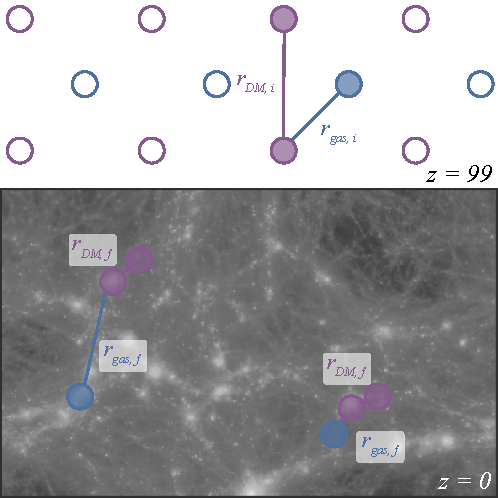
\includegraphics[width=\columnwidth]{figures/kspafig_small.pdf}
    \vspace{-0.5cm}
    \caption{The matching procedure between initial and final conditions
    illustrated. The top panel shows the $z=99$ initial conditions, where
    every particle finds its nearest dark matter neighbour. The bottom
    panel shows the distances between those particles at $z=0$. For the
    fiducial result, each particle actually finds the three nearest 
    neighbours in the initial conditions and takes the median at $z=0$
    of these distances (see text for explanation) but this is omitted
    in this simple picture for brevity.}
    \vspace{-0.5cm}
    \label{fig:kspafigsmall}
\end{figure}

Our approach to quantifying the large-scale impact of feedback is to develop
a simple and robust metric that directly captures the displacement of the gas
owing to feedback. This `spread' metric, illustrated in Figure
\ref{fig:kspafigsmall}, works as follows:

\begin{enumerate} 
	\item For every particle $i$ in the initial conditions, find the nearest
          $n$ dark matter neighbours $j$ (with $n=3$ for the fiducial result).
	\item In the final conditions, match all remaining baryonic particles
	      with their initial conditions progenitor (in this case, stars are
	      matched with their gas progenitor).
	\item In the final conditions, find the distance $r_{ij}$, i.e. the
	      distance between the particle and its original neighbours. The spread metric for
	      this particle is then given as the \emph{median} of these $n$
	      distances.
\end{enumerate}

\begin{figure}
    \centering
    \includegraphics{report/figures/s50j7k/dark_matter_distance_figure_s50j7k.pdf}
    \vspace{-0.5cm}
    \caption{Shows the distribution of final-state distances from the spread
             metric for dark matter in the full \simba{} model run. This distribution
             is relatively unchanged by the choice of sub-grid
             model, and the effects of the back-reaction of baryonic physics on dark
             matter is out of the scope of this work. The distribution is split
             between particles that lie within halos and those that lie outside, with
             this being an approcimately even split at $z=0$. Lines are over-plotted
             to show the maximal distance between any two dark matter particles at $z=0$,
             approximately $0.5\hmpc{}$, and twice the maximal virial radius of any halo 
             in the box, which is approximately $1.3\hmpc{}$. The inset figure
             shows the inner $0.5\hmpc{}$ of the distribution, and has a line over-plotted
             for the mean inter-particle separation in the initial conditions (MIPS)
             of approximately $0.1\hmpc$. The fainter lines show how the short-distance
             distribution changes when taking the average over a number of initial nearest
             neighbours; dashed gives the metric with no median (i.e. only one nearest
             neighbour), and the dotted line shows the case for a median over 9 neighbours.
            }
    \vspace{-0.5cm}
    \label{fig:dmonlyspread}
\end{figure}

The `spread' metric is presented first for dark matter in Figure \ref{fig:dmonlyspread}.
The simplest metric here clearly is simply to use the nearest neighbour in the
initial conditions, rather than the median over $n$ initial neighbours. The
choice of $n=3$ was made primarily to ensure that the dark matter results were
robust when comparing matter inside and outside of halos. For a given
dark matter particle pairing, a large distance between two neighbours
would be `double counted' for the case where one neighbour makes it into
a halo and one remains outside, contributing the large distances to both
bins. Choosing $n=3$ enables the median result to actually represent the
distance to a full particle, and removes the problem of the double counting
for the nearest neighbour. The overall distributions of distances, however,
were not changed much by this choice. It does increase the contrast in the
dark matter images in Figure \ref{fig:bigdistanceimage}, with more substructure
being picked up in the low-distance particles, and more diffuse structure in the
large-distance particles, with an increasing number of neighbours.

\begin{figure*}
    \centering
    \vspace{1cm}
    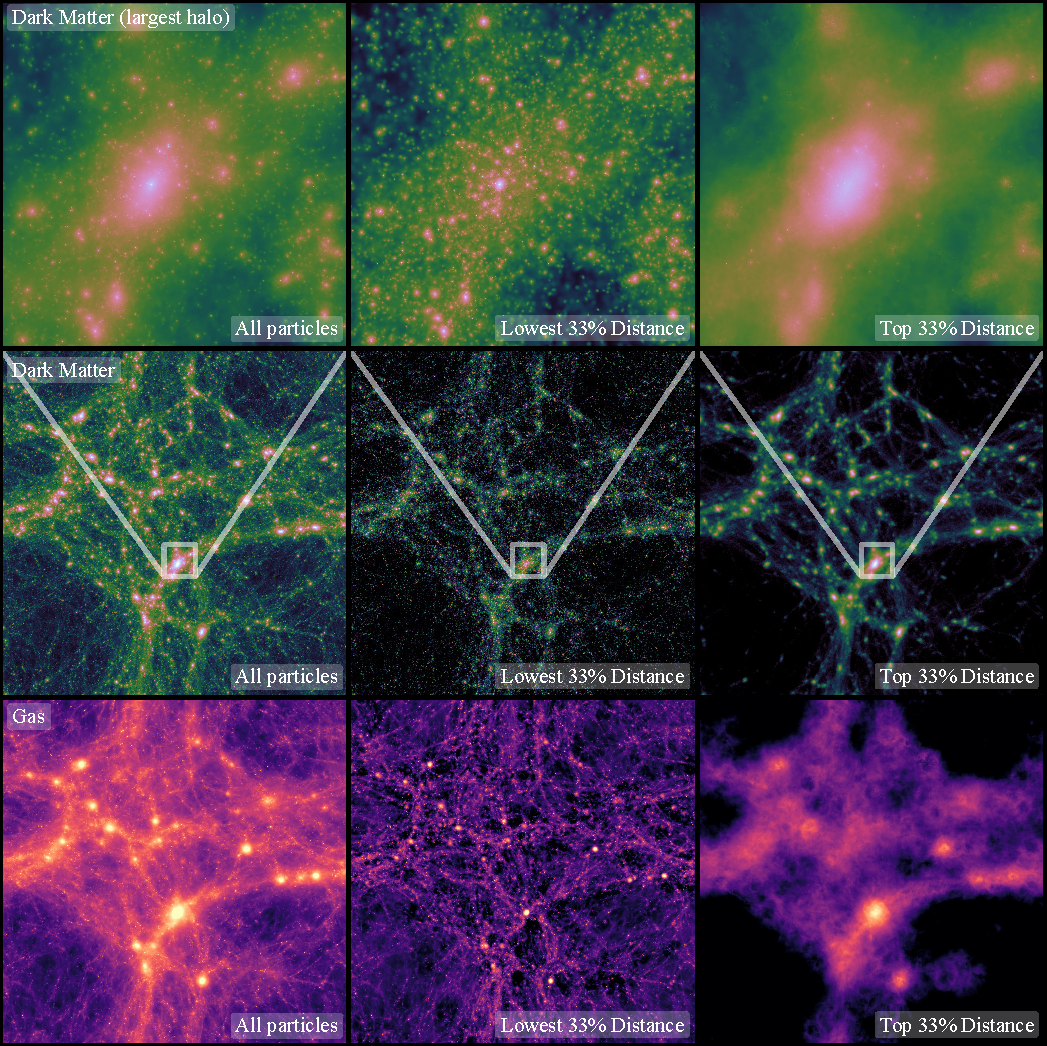
\includegraphics[width=\textwidth]{report/figures/distance_figures_3.pdf}
    \caption{The three rows show the following selections of particles (from top to bottom):
        the dark matter present in the largest halo, and surrounding it (this is a $4.5\hmpc{}$
        cube centered around the halo centre, which has a virial radius of approximately $1.3\hmpc{}$);
        all dark matter particles in the box; and all gas particles present in the box. All images
        are shown in the final state of the simulation at redshift $z=0$. Each column then shows
        (from left to right): all particles that are in the volume; the particles that have spread
        the least, selecting the first 33\% from the histogram figures; and the particles that have
        spread the 33\% most. For the dark matter, these cuts correspond to particles that have travelled
        less than $0.1\hmpc{}$, and greater than $0.25\hmpc{}$ respectively. For the gas, these numbers
        increase to $0.45\hmpc{}$ and $1.25\hmpc{}$ respectively due to the larger spread that these
        praticles expereice. Each image has smoothing lengths generated to encompass $32$ nearest
        neighbours, as is used in the \simba{} simulations, and smoothing lengths are kept consistent
        across columns; i.e. they are not re-smoothed. All images in a given row also use the exact
        same (logarithmic) normalisation and colour map to enable comparisons. Note how even with this
        extremely conservative cut there is a significant difference between the images, with sub-structure
        picked out by the low-distance cut and large-scale structure for the large-distance cut.}
    \vspace{1cm}
    \label{fig:bigdistanceimage}
\end{figure*}


Figure \ref{fig:feedbackpic} visualizes how this metric looks in our \simba{}
simulation. This metric shows the extreme distances that feedback processes
can cause baryons to be ejected to. Note that the colour bar for distance
shows separations of over $10\hmpc{}$. The background gas density map shows
the positions of halos in the simulation; note that the majority of particles
that are ejected to large distances (relative to their dark matter) end up
far outside any of the large halos. The metric also shows that the central
galaxies of the halos are predominantly made up of tightly bound baryons and
dark matter (i.e. the baryons in these halos have not moved very far relative
to their closest dark matter neighbour in the initial conditions). This again
re-enforces the view that central galaxies initially form out of the gas made
up of their halo, but feedback processes cause outflows of gaseous material
that both pollutes the CGM and IGM surrounding that halo and may find its way
into other halos.

\subsection{Baryon Spreading in \simba{}}

\begin{figure}
    \centering
    \includegraphics{report/figures/s50j7k/distance_plot_split_by_component.pdf}
    \vspace{-0.5cm}
    \caption{The distance metric histogram, now including gaseous matter. Note how,
    compared to the dark matter, the distributions for gas inside halos and outside
    halos are significantly different, with gas that originated in lagrangian regions
    being preferentially moved to larger distances than gas on average. Note that only
    10\% of the gas in the entire simulation is in halos at $z=0$. Gas can be blown
    out to $12\hmpc{}$, approximately 10 times the virial radius of the largest halo
    in the box.
    \blue{TODO: Change the normalisation here to be the same as above}.}
    \vspace{-0.5cm}
    \label{fig:distbaryon}
\end{figure}

Now considering the baryons in the simulation in Figure \ref{fig:distbaryon}.

\begin{figure*}
    \centering
    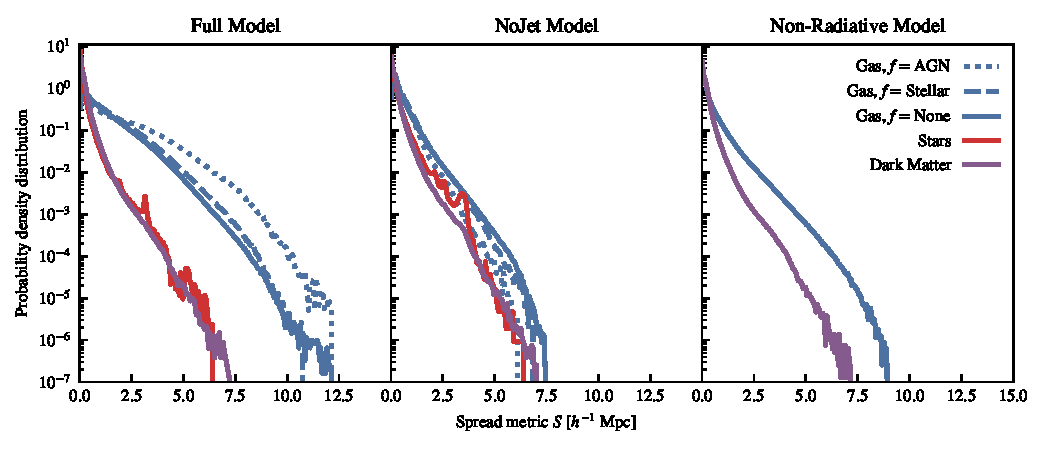
\includegraphics[width=\textwidth]{figures/neighbour_analysis_feedback_histogram_combined.pdf}
    \vspace{-0.7cm}
    \caption{
        The (normalised) distribution of distances for all particles $i$ to
        the nearest neighbour $j$ in the initial conditions, split by particle
        type. This is shown for the $z=0$ particle distribution in the
        reference model (left), \nojet{} model (center), and a non-radiative
        run (right). Splitting the particles by those that have been
        involved in feedback events in this figure shows that the further
        out a particle has been blown the more likely it is to have been
        directly involved in a feedback event for the reference model. Also note
        the vertical $0.5-1$ dex offset for gas compared to dark matter even in
        the \nojet{} run. \blue{TODO: Change the normalisation here}.
    }\label{fig:feedbackdistance}
\end{figure*}

In Figure \ref{fig:feedbackdistance} (left panel) the distribution of
distances in the reference model is shown. Note how similar the stellar
distribution is to the dark matter distribution even though strong feedback
is included. From this we conclude that star particles are mainly formed out
of tightly bound gas (this is ensured almost by construction due to the
density criterion in the sub-grid model) that is unable to separate
dynamically from the dark matter. Also, the peak of star formation is far
before redshift $z=0$ and so it is unsurprising that the stellar dynamics
have relaxed back to something similar to the dark matter despite starting
out life as gas. The maximal distance of around $6\hmpc{}$ is expected, as it
is about three times the virial radius of the largest halo in the simulation;
a pair of initially neighbouring particles can end up on opposite sides of a
given halo. Matter that remains in a gaseous state, on the other hand, can be
blown out to very large distances (over $12 \hmpc{}$).

Comparing to the \nojet{} run in Figure \ref{fig:feedbackdistance}, it is clear
that the jets have a significant impact on the distances to which particles
are spread. These two plots show directly the issue of entrainment that was
raised earlier; the tail is expanded to include lots of gas that was never
tagged as having been included in any feedback event.

The significant difference in the dynamics between the \nojet{} run and the
reference model is surprising. Less than $0.4\%$ of gas particles in the simulation
have ever interacted directly with the AGN jets; this has been enough
to completely separate the majority of the gas from the dark matter dynamically.
Such a high degree of separation points to huge amounts of gas being entrained
by these powerful jets. It is not simply the case that higher mass ($M_H >
10^{11} \msolar{}$) halos are quenched internally reducing their star formation
rate; the energetics and dynamics of the CGM and IGM are significantly altered
leading to a much more complex interaction between the turn-off of the
galaxy stellar mass function (GSMF) and the power of the AGN jets.

The final contrast to highlight is the difference between the \nojet{} and
non-radiative model. The non-radiative model shows increased distance between
gas particles and their associated dark matter neighbour compared to the
\nojet{} run; this is likely due to the lack of cooling preventing particles
that lie in small halos from remaining as tightly bound.

\begin{figure}
    \centering
    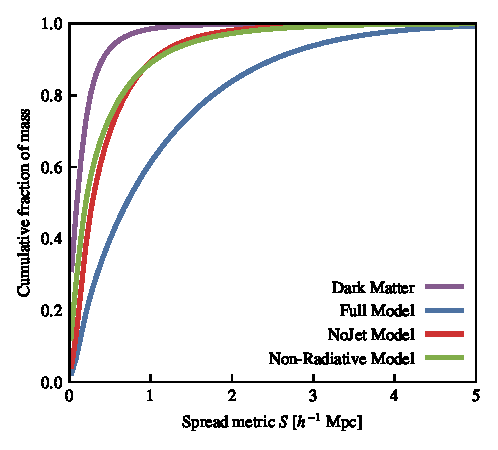
\includegraphics{figures/cumulative_histogram_comparison.pdf}
    \vspace{-0.7cm}
    \caption{Cumulative version of Fig. \ref{fig:feedbackdistance} that
    shows the gas distribution for the three models alongside the dark
    matter from the full model.}
    \label{fig:cumulativehistogram}
\end{figure}

In Fig. \ref{fig:cumulativehistogram} we show the cumulative version of Fig. 
\ref{fig:feedbackdistance} to show that it is not a negligible amount of mass
that is entrained by the full model out ot large distances. Only 90\% of gaseous
mass is constrained within $3\hmpc{}$.

These results show that gaseous and stellar matter can be transferred out
to significantly further (by $z=0$) than is assumed by typical zoom-in simulation
suites. For example, the Latte \citep{Wetzel2016} suite uses an exclusion region
for high resolution particles of around $1.5 \hmpc{}$. Whilst they do not find
contamination (possibly due to refinement criteria) of low-resolution particles
into the high-resolution region, the above metrics suggest that perhaps this is
a more numerical, rather than physical, effect; low resolution particles are
not present due to a lack of sub-grid physics in the unrefined region.

\begin{figure*}
	\centering
	\vspace{0.5cm}
	\includegraphics{figures/fancy-figure.pdf}
 \caption{ This visualisation shows two epochs at once, simultaneously
 showing the initial conditions (in blue and red) and the final simulation
 volume at redshift $z=0$ in white/grey. The blue and red show the positions
 of the gas and dark matter (respectively) \emph{in the initial conditions}
 for particles that reside in selected haloes at redshift $z=0$. The overlaid
 white/grey map shows the dark matter at redshift $z=0$ to enable comparisons
 between the initial and final comoving positions for various bound
 structures. For each selected halo, the dashed black circles show their
 virial radii as defined in \S \ref{sec:simba}. For some haloes in crowded
 regions, we have overlaid a circle and arrows showing which blob of dark
 matter and gas in the initial conditions collapses to form this halo.
 Finally, for each halo we show a small bar chart showing how their gas is
 composed from Lagrangian components, as described later in the text. The
 blue bar shows the fraction of gas in each halo that originated from that
 haloes own Lagrangian region, the red bar shows the gas from another haloes
 Lagrangian region, and the purple bar shows the fraction of gas that
 originated outside any Lagrangian region. This figure illustrates the
 significant differences in origin between the gas (blue) and dark matter
 (red) for these selected haloes of various masses. We also see how the
 environment of each halo changes its Lagrangian make-up. In particular,
 group 431 shows a large baryonic component originating from the Lagrangian
 region of another halo, with this halo entering a small cluster environment
 near the end of the simulation. Note that individual regions are
 colour-mapped separately, i.e. the intensity of colour for a single halo is
 unique to that halo only, as to enable all Lagrangian regions to be seen.
 Without this choice, the structure for the lower mass haloes would be
 completely washed out.}
	\vspace{1cm}
	\label{fig:bigtransferpic}
\end{figure*}


\begin{figure*}
    \centering
    \vspace{1cm}
    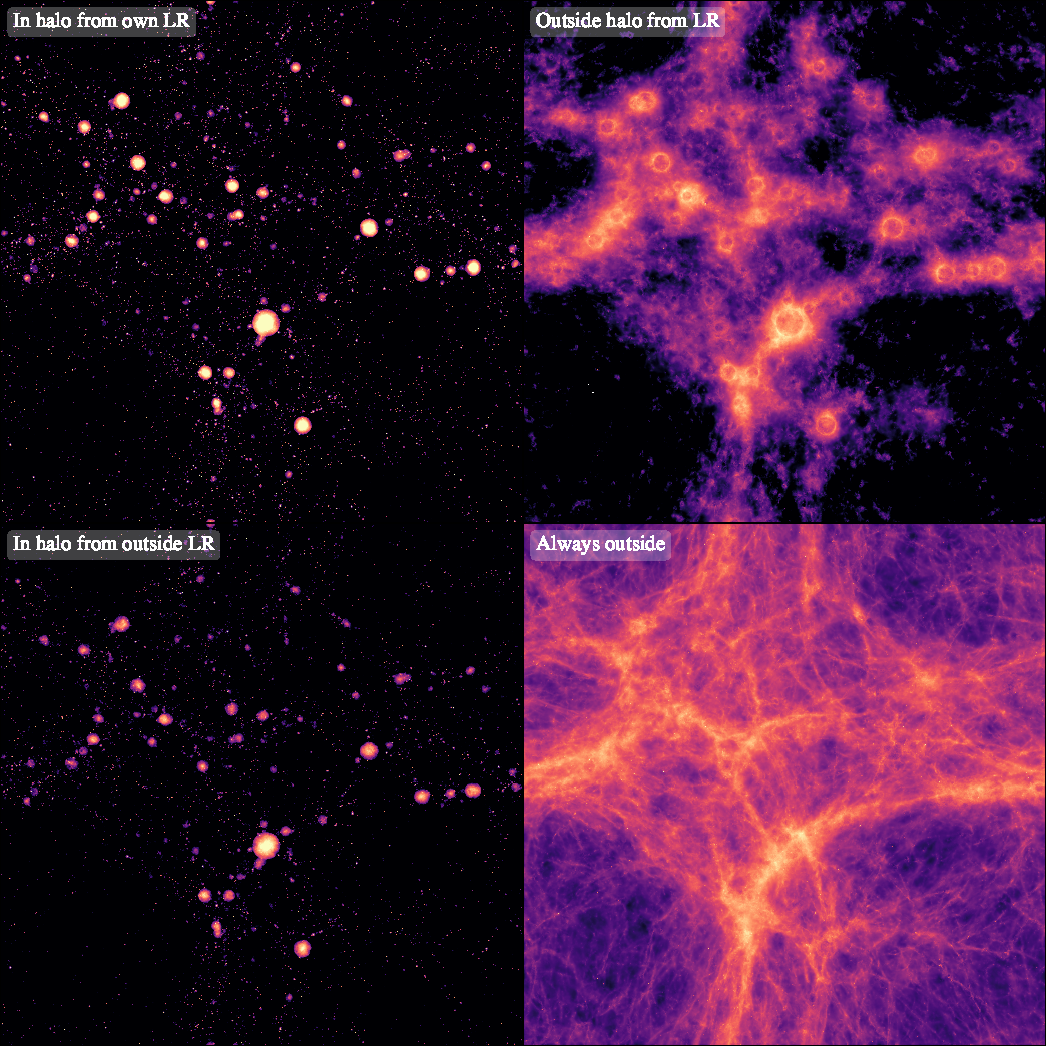
\includegraphics{figures/s50j7kAHF/four_images_magma_AHF.pdf}
    \caption{Gas distribution in the fiducial \simba{} model for the full
    $50\hmpc{}$ volume, split by the following Lagrangian components
    (clockwise, starting from top left): particles that began in Lagrangian
    regions at $z=99$ and have remained in the associated haloes at $z=0$;
    particles that began in Lagrangian regions and ended up outside of the
    destination halo; particles that began outside any Lagrangian region and
    ended up outside any halo; and particles that ended up in a halo but
    originated outside any Lagrangian region. All images are shown with the
    same (logarithmic) colour-map and normalisation and taking their linear
    sum would reproduce the full gas distribution at $z=0$. Gas particles
    that began in Lagrangian regions but ended up outside of haloes (top
    right) show a striking similarity to the distribution of gas with the
    33\% highest spread distance shown in Fig.~\ref{fig:bigdistanceimage}.
    As expected, particles that began outside of Lagrangian regions and
    remained outside of haloes (bottom right) trace the filaments and voids.}
    \vspace{1cm}
    \label{fig:lrtransfer}
\end{figure*}

\section{Lagrangian baryon transfer}
\label{sec:transfer}

We have explored the relative motion of dark matter and baryons using a
particle-level metric, showing that AGN jets in the \simba{} cosmological
simulations can spread baryons up to $12\hmpc{}$ relative to the neighbouring
dark matter. In this section, we consider the movement of baryons relative to
dark matter haloes and their corresponding Lagrangian regions. The definitions of
haloes and Lagrangian regions used here are described in \S \ref{sec:simba}.

This topic has been considered recently by \citet{Liao2017}, where they used
a $10\hmpc{}$ non-radiative simulation to show that the gas in haloes may
originate from different places than the dark matter in those same haloes in
the initial conditions.

\subsection{The different origins of baryons and dark matter in haloes}

Fig. \ref{fig:bigtransferpic} illustrates the mixed origins of the gas and
dark matter components in bound structures at $z=0$ by showing simultaneously
the initial and final states of the simulation. A common trend for all haloes
is a shell of gas around the main dark matter component in the initial
conditions, showing that gas in general is able to collapse further (due to
cooling and other processes) than the dark matter, which is unable to lose
angular momentum as efficiently. This is consistent with the larger values of
the spread metric for gas in haloes relative to the dark matter in haloes, as
shown in Fig. \ref{fig:distbaryon}.

The origin of the dark matter in the initial conditions corresponds exactly
to our definition of Lagrangian region for that component in \S
\ref{sec:simba}. These Lagrangian regions have very complex shapes, with
larger haloes tending to have more spherical Lagrangian regions, as can be
seen with the largest halo in the box (Group 0) in Fig.
\ref{fig:bigtransferpic}. These complex non-spherical shapes are why we
chose to identify our Lagrangian regions for gas through neighbour searching,
as other methods (e.g. constructing a convex hull enclosing all dark matter
particles that end up in a given halo) would not allow us to capture the
surprisingly intricate structure that is at play here.

There are many possible reasons for the complex shapes that we see here.
Consider a simple case where we have one `main' halo, and a satellite that is
being accreted. The gas and dark matter in the satellite galaxy have several
potential fates. For instance, when accreting onto the main halo, the gas in
the satellite may be shock heated, and stalled in the CGM, with the dark
matter being able to continue to move towards the center of the main halo.
This process dynamically separates the dark matter and gas, and now the gas
may have several fates; it could be pushed out in a feedback event, rise out
of the halo due to buoyancy, or fall to the centre of the halo after cooling
and re-join the dark matter. Once the gas has been removed from the CGM into
the IGM, it is free to be picked up by other passing galaxies.

The other possibility for the fate of this substructure is the dark matter
failing to accrete onto the central. In this case, the dark matter continues
moving out into the IGM, with the gas being shocked and captured by the main
halo. It is this complex difference in assembly between dark matter and
baryons, due to the latter behaving as a collisional fluid, that we aim to
capture here.

\subsection{Computing transfer between Lagrangian regions}

Given the definitions of haloes and Lagrangian regions in
\S \ref{sec:simba}, it is possible to classify every particle in the
simulation according to their Lagrangian ID and halo ID (if any) in the
initial and final conditions. The algorithm is as follows:

\begin{enumerate}
	\item ID match all particles between the initial and final conditions, including
	      star particles (these are matched to their gas progenitor). Black holes are ignored in this analysis since globally they represent a minimal amount of mass.

	\item Every particle at $z=0$ has several possible final states and origins, based on its halo ID ($i$) and Lagrangian region ID ($j$):
	      \begin{itemize}
	            \item Particle resides in  halo ($i \neq -1$)
	            \begin{itemize}
	           		\item Particle originated in the same Lagrangian region, $j = i$
	           		\item Particle originated outside any Lagrangian region, $j \equiv -1$
	           		\item Particle originated in some other Lagrangian region, $j \neq i$
	            \end{itemize}
	            \item Particle resides outside of any halo ($i \equiv -1$)
	            \begin{itemize}
	            	\item Particle originated outside any Lagrangian region, $j = i$
	            	\item Particle originated in some Lagrangian region, $j \neq i$
	            \end{itemize}
	      \end{itemize}
	      
	\item For every halo and Lagrangian region, the mass originating from each
	      of the above components is computed and stored.
\end{enumerate}



A visualisation of this particle classification scheme is shown in
Fig.~\ref{fig:lrtransfer}, where we split the gas distribution in the
\simba{} $50\hmpc{}$ box into the four main Lagrangian components that we
consider in the remainder of this paper. Considering each panel clockwise
from the top left, we select first the gas that is in the same halo at
redshift $z=0$ as the Lagrangian region that it originated in. As expected,
we see a population of spherical shapes corresponding to every halo in the
box, with their sizes corresponding to $R_{\rm vir}$ as defined by AHF. The
centers of haloes, where the gas is densest, are the brightest.


In the top right panel we have the gas that is outside any halo at $z=0$, but
is assigned to a Lagrangian region at $z=99$; this is the gas that should
have ended up in haloes by the end of the simulation if the baryonic matter
was also collisionless. We see that this component traces gas primarily
around massive haloes, resembling the large-scale bubbles that the AGN jets
power in \simba{} \citep{Dave2019}. Note that some of this gas piles up just
outside of haloes due to the somewhat arbitrary boundary defined by the
virial radius of haloes. This gas resides primarily in filaments, with some
reaching out into the voids.

In the bottom right panel, we visualise the gas that begun outside any
Lagrangian region and resides outside any halo at redshift $z=0$. This gas
traces the majority of the filamentary structure, and shows all of the
structure in the voids. 

Finally, in the bottom left panel, we have the gas that is in haloes at $z=0$
but originated from outside any Lagrangian region. As expected, this shows a
very similar structure (albeit less bright) to the gas that resides in its
own halo (top left), but this component originates from regions where the
dark matter now resides outside of haloes. This gas is likely dragged into
these bound structures by cooling flows, while the dark matter
is not able to lose angular momentum quickly enough to assemble by $z=0$.




\subsection{Transfer in a non-radiative Model}

\begin{figure}
	\centering
	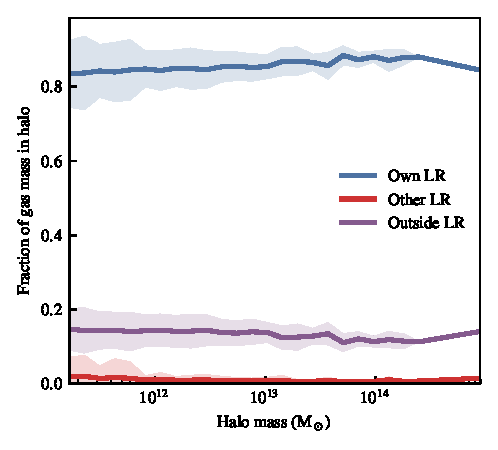
\includegraphics[width=\columnwidth]{figures/s50gadget/component_fraction_vs_halo_mass_gas.pdf}
	\vspace{-0.7cm}
 \caption{ The fraction of baryonic mass originating from each Lagrangian
 component in the non-radiative model (i.e. without sub-grid physics) is
 shown as a function of redshift $z=0$ halo mass. The gas particles are
 binned by their origin, with the baryons originating from their own
 Lagrangian region shown in blue, the Lagrangian region of other haloes
 (red), and outside of any Lagrangian region (purple). Shaded regions show
 the $1\sigma$ scatter in a given bin, which is given by one standard
 deviation of variation. The lines represent the mean value within each bin.
 Approximately 85\% of the baryonic mass of a given halo originates from its
 own Lagrangian region, showing very little transfer of baryons from either
 outside or from another Lagrangian region. This is provided for comparison
 to the full model result in Fig. \ref{fig:maintransferresult}.}
	\label{fig:nonradiativetransfer}
\end{figure}


Before considering the numerical results of the full model, we first present
the non-radiative simulation as a null model to investigate the effects of
hydrodynamics alone. In this case, we run the simulation without cooling,
star formation, or feedback, only including hydrodynamics, cosmology, and
gravity. In Fig. \ref{fig:nonradiativetransfer} we present the fraction of
baryonic mass for each halo contributed from each Lagrangian component, as a
function of halo mass. The blue line shows the fraction of mass in each halo
from its own Lagrangian region (top left in Fig. \ref{fig:lrtransfer}), the
red shows transfer into a halo from another Lagrangian region, and the purple
line shows the fraction of baryonic mass from outside any Lagrangian region
(bottom left in Fig. \ref{fig:lrtransfer}). There is no dependence on halo
mass (as the simulation is effectively scale-free above some resolution
limit), and apart from some small level of transfer from outside any
Lagrangian region (of around $10-15\%$), the baryonic mass in each halo
consists of that which originated in its own Lagrangian region.

The difference in origins of the baryons in the final haloes, from
hydrodynamical effects alone, is then around the $10-15\%$ level. This is
close to the 25\% level of segregation between gas and dark matter reported
by \citet{Liao2017} (who also used a non-radiative simulation), with the
difference likely rooted in the definitions that we use. We consider the
fraction of gas particles in the final redshift $z=0$ halo whose initially
pairing dark matter is also resident in that halo; hence what we are really
counting is the `contamination' of the halo by gas particles from outside of
its Lagrangian region. \citet{Liao2017} count all particles in the final
halo, treating gas and dark matter equally, then finding all particles that
were gas-dark matter pairs in the initial conditions. Their higher level of
segregation is expected due to contributions from dark matter particles that
are resident in a halo but whose initial gas pair is not. Fundamentally this
represents the difference in our approaches; here we are interested in
treating the dark matter as a ground source of truth, and asking if the gas
nearest to that dark matter follows it into the same haloes.
\citet{Liao2017}, on the other hand, were interested in treating \emph{all}
occupants of the final halo as the ground source of truth, and asking what
differences there were in their origin.

The causes for our contamination here are less clear than in the case of
\citet{Liao2017}; we would report a halo that has had gas only \emph{removed}
as being completely uncontaminated, and hence stripping of gas is
an unsatisfactory explanation of these differences. The likeliest explanation
for the contamination in this case is that the baryons and dark matter go through
a phase of mixing as they enter the cosmic web, before going on to fully
collapse into bound structures.


\subsection{Transfer \emph{into} haloes}
\label{sec:transferinto}


\begin{figure*}
	\centering
	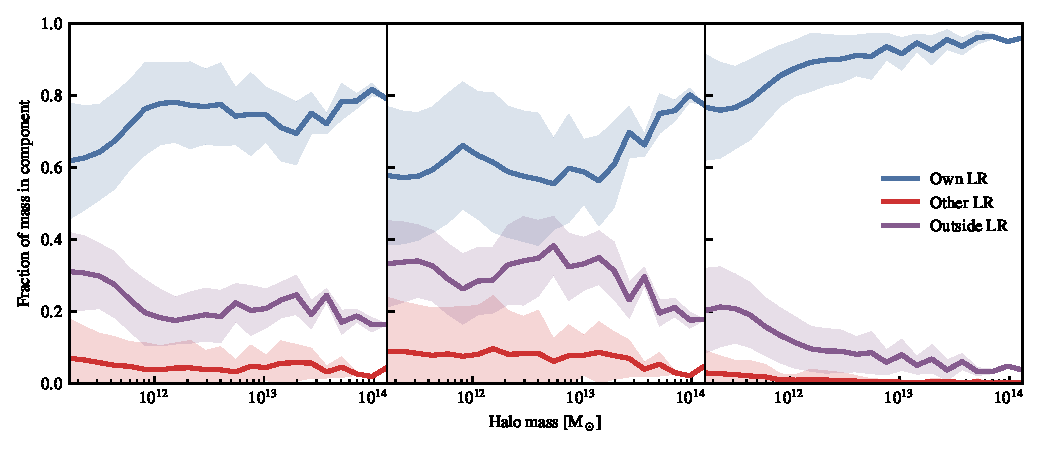
\includegraphics{figures/s50j7kAHF/component_fraction_mixed.pdf}
	\vspace{-0.7cm}
	\caption{
  The fraction of baryonic mass in haloes at $z=0$ originating from their own
  Lagrangian region (blue), the Lagrangian region of other haloes (red), and
  outside of any Lagrangian region (purple), shown as a function of $z=0$
  halo mass for the fiducial \simba{} model. We consider all baryons in
  haloes (left) as well as their gas (center) and stellar (right) components
  separately.
	}
	\label{fig:maintransferresult}
\end{figure*}

Moving on to the full \simba{} model, we consider again the fractions of
baryonic mass as a function of halo mass, split by Lagrangian component. Fig.
\ref{fig:maintransferresult} shows three panels: the left panel shows all
baryons, the centre shows only gas, and the right panel shows the
contribution from only the stars. The lines are coloured the same as the
non-radiative model shown in Fig. \ref{fig:nonradiativetransfer}. Now that we
have introduced scale into the simulation through density-dependent energy
injection mechanisms, these components scale with halo mass. The general
trend is that for an increasing halo mass, a Lagrangian region is able to
hold on to more of the original baryonic mass, with this flattening off
around $M_H = 10^{12} \msolar$. For a given halo, significantly more of the
gaseous mass originates outside the original Lagrangian region as compared to
the stellar mass ($\sim 40 \%$ versus $\sim 10 \%$). The transfer between
haloes is at around the $\sim 10\%$ baryonic mass level, with this transfer
predominantly originating from the gaseous component, as compared to the
stellar component. This combines nicely with the distance metrics shown in \S
\ref{sec:feedbackmetrics}, which showed that the dark matter and stars have
very similar dynamics and hence should be similarly well bound.


This transfer into, and between, Lagrangian regions can have several physical
origins. The first, as shown in the non-radiative run, is caused by the
collisional dynamics of the gas preventing gas from following the dark matter
in all cases. We found that this can account for up to 15\% of the baryonic
mass of a bound structure at redshift $z=0$ originating from a different
region than the dark matter (see Fig. \ref{fig:nonradiativetransfer}), but this
could not account for any \emph{inter-Lagrangian} region transfer.

The galaxy formation sub-grid model clearly has a significant effect on the
baryonic make-up of haloes at redshift $z=0$. The fraction of mass from
outside any Lagrangian region has increased to 20-40\%. This increase is
explained by the inclusion of sub-grid cooling and feedback processes, with
the baryons now able to cool before accreting and lose angular momentum at a
much higher rate than the dark matter component is able to.

Around 10\% of the baryonic mass of haloes is now made up of gas that has
experienced inter-Lagrangian transfer. It is important to recall that this is transfer
between bound structures at redshift $z=0$, and that it only takes into account
the initial and final conditions of the simulation; this analysis does not
consider the complete history of these particles.

The transfer between haloes has several possible sources: stripped gas from
nearby galaxies that are still classified as their own bound structures at
redshift $z=0$, gas that has been expelled from galaxies through stellar
winds or AGN feedback and re-captured by a halo, and transfer due to boundary
effects caused by the complex shapes of Lagrangian regions according to the
definition adopted. With the non-radiative simulation showing zero transfer
between haloes, and there being little transfer before $z=2$ in the fiducial
model (see below in Fig. \ref{fig:ltzevo}), we believe that the contribution
from pure dynamics alone to inter-Lagrangian transfer is likely very small.
When repeating this analysis with the \nojet{} run, the inter-Lagrangian
transfer is reduced, but still remains at the 10\% level. The feedback events
that power this transfer must be dominated by the expulsion (or alternatively
preventative pathways) from stellar winds and the residual thermal AGN
feedback.

A given mass bin contains haloes that entertain a range of 10x in transfer,
which is likely dependent on environment. Future work should investigate in more detail
the physical mechanisms driving the scatter in these relations.

The level of transfer above a halo mass of $10^{13} \msolar{}$ must be
interpreted carefully, as there are very few haloes above this mass present
in the box (less than 50), with the small scatter being misleading. It is
also important to note that the shaded regions in Fig.
\ref{fig:maintransferresult} represent the $1\sigma$ scatter in a given bin
and explicitly do \emph{not} include any dispersion that would occur from a
finite sampling of haloes or halo assembly bias.

\subsection{Redshift evolution of transfer into haloes}

\begin{figure}
    \centering
    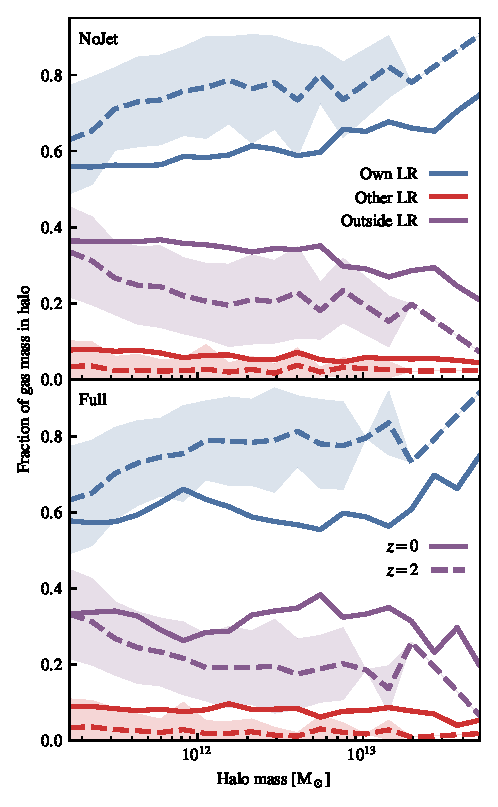
\includegraphics[width=\columnwidth]{figures/component_fraction_multi_z.pdf}
    \vspace{-0.7cm}
    \caption{The fraction of gas mass in haloes at redshift $z=0$ (solid) and
    redshift $z=2$ (dashed) as a function of halo mass at that redshift, split by
    Lagrangian component. Scatter is shown only for the $z=2$ results. The top panel
    shows the results from the \nojet{} simulation, with the bottom showing the
    full \simba{} model.}
    \label{fig:ltzevo}
\end{figure}

To further investigate the origin of the inter-Lagrangian transfer, in Fig.
\ref{fig:ltzevo}, we consider the \nojet{} model and show how the gas in
haloes at redshift $z=2$ is composed in this and the full \simba{} model.

We see that both the \nojet{} and \simba{} models broadly reproduce the same
fractions of gas in each Lagrangian component, with some interesting
differences. In the full model, a higher fraction of the halo gas originates
from inter-Lagrangian transfer than the \nojet{} model at all masses, with no
change in the shape of this function observed. The level of inter-Lagrangian
transfer is increased by around $25-50\%$ such that it represents
approximately $15\%$ of the gaseous mass in the halo, with the \nojet{}
results showing an inter-Lagrangian fraction of $\sim10\%$. The fraction of
gas originating outside of any Lagrangian regions shows a dip at around
$10^{12}\msolar{}$ being removed in the \nojet{} model, however this is well
within the scatter that we observe in the full model results.

All of this is despite both models producing very different $z=0$ halo baryon
fractions (see Fig. \ref{fig:baryonfraction} for the full model; the \nojet{}
model produces baryon fractions at approximately the cosmic mean for all halo
masses above $\sim10^{11}\msolar{}$). For a further investigation, halo matching
should be performed between the two models and individual cases compared, but
this is out of the scope of the current work.

The fraction of gas in haloes originating from the different Lagrangian
components shows a closer match at $z=2$, with the shape and
normalisation of all components being well within the reported scatter. The
higher-mass end of these results ($M_H > 10^{13}\msolar{}$) also lacks
objects here, with there being even fewer in this mass range than at $z=0$.

We see that between redshift $z=2$ and $z=0$ a change in the slope
of these functions takes place, and that the level of inter-Lagrangian transfer
increases significantly. The fraction of gas originating from the Lagrangian 
regions of other haloes increases by a factor of two (or more) at all halo
masses, with the fraction of transfer from outside Lagrangian regions remaining
constant or again increasing by a factor of two dependent on the resident halo mass.

All of this must be explained within the context of very different baryon
fractions for all haloes at $z=0$. One possibility is that the majority of
gas gained from outside of a haloes own Lagrangian region remains in the CGM,
with very little of it making it into the disk (this is supported by the very
low fraction of halo stars that originate from transfer, see Fig.
\ref{fig:maintransferresult}). This gas can then be swept out of the halo
either by stellar winds or (ejective) AGN feedback. Alternatively, if the
main pathway for feedback is preventative, and the gas outside of haloes is
well mixed, then this assembly of baryons would be curtailed equally for all
Lagrangian components. A further investigation of these transfer properties
(considering differences between the galaxy disks and the CGM) would be well
suited for follow-up work using higher resolution simulations.

\subsection{Transfer \emph{out} of Lagrangian Regions}

\begin{figure}
	\centering
	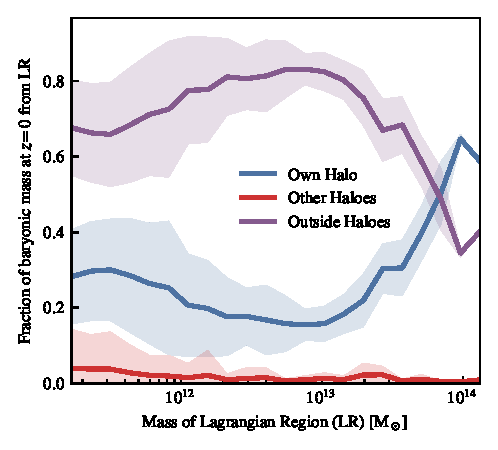
\includegraphics{figures/s50j7kAHF/inverse_component_fraction.pdf}
	\vspace{-0.7cm}
 \caption{The fate of gas that begins in Lagrangian regions, as a function of
 initial Lagrangian region mass. The blue line shows the fraction of baryons
 that reside in the halo that defines the Lagrangian region at redshift
 $z=0$, the red line shows the the fraction of baryons that lie in a
 different halo, and the purple line shows the baryons that lie outside of
 any halo at redshift $z=0$. All but the most massive objects in the box
 struggle to retain more than 30\% of their baryons due to various factors,
 see the text for details. The fraction of mass retained in the corresponding
 halo (blue) is the lowest in the mass range $10^{12} - 10^{13}\msolar{}$.}

	\label{fig:transferoutoflrs}
\end{figure}



Let us now consider the fates of baryons that begin their lives in Lagrangian
regions. This material has three possible fates, as shown in Fig.
\ref{fig:transferoutoflrs}: it can end up in the same halo as the dark matter
from that Lagrangian region (blue line), in another halo (red line), or
outside of any halo in the IGM (purple line). Here, we we plot the fraction
of LR mass at $z=0$ from each component as a function of their Lagrangian
region mass (this is the sum of the baryons and dark matter contained within
that Lagrangian region). The Lagrangian region mass is somewhat higher than
the eventual halo mass due to the baryon fractions of redshift $z=0$ haloes
being below the cosmic mean. We see that, below a halo mass of
$10^{13.5}\msolar{}$, only around 20-30\% of the baryons initially present in
the Lagrangian region make it in to the halo by $z=0$. Only above a halo mass
of $10^{13.5}\msolar{}$ do haloes become strong enough attractors to retain
the majority of their baryons. Despite the clear trend, this result is
somewhat uncertain due to the very small number of these very large haloes
present in our $50\hmpc{}$ box. On top of this initial structure, we see that
there is a dip in the retained fraction of baryons between $10^{12}$ and
$10^{13}\msolar{}$. We speculate that this is due to the increased efficiency
of AGN feedback in haloes in this mass range, allowing for more gas in
central objects to be expelled, however making a direct connection would
require significant investigation. It is worth noting that without the AGN
jets (i.e. in the \nojet{} run), the baryon fraction of haloes in this mass
range is approximately $f_b / f_{b,c} = 1$.

Finally, we find that up to 10\% of the Lagrangian region gas of low-mass
haloes ($<10^{12} \msolar{}$) can be transferred to other haloes, decreasing at
higher masses. A larger cosmological volume with more objects is required for
a full study of objects at masses higher than $M_H > 10^{13}\msolar{}$, but
these trends point towards inter-Lagrangian transfer being fuelled by
accretion of gas that is either expelled or stripped from lower mass haloes
by higher mass objects. A plausible physical scenario is that early
feedback leading up to redshift $z=2$, where star formation (and hence
stellar feedback) peaks, expels significant quantities of gas from lower mass
haloes that can then be swept up at later times from the IGM by all haloes.
Higher mass haloes at this redshift may have a strong enough gravitational
potential to enable their stellar winds to be more efficiently recycled,
preventing them from being sources of inter-Lagrangian transfer.

The combination of the baryons that are retained by haloes (Fig.
\ref{fig:transferoutoflrs}) and the baryons that they manage to accrete from
sources outside their Lagrangian region (Fig. \ref{fig:maintransferresult})
is seen in the baryon fraction of haloes, shown in Fig.
\ref{fig:baryonfraction} split by Lagrangian component. Here, we split the
overall baryon fraction (relative to the cosmic mean) into three Lagrangian
components, coloured by the baryons from the haloes own Lagrangian region
(blue), other Lagrangian regions (red), and from outside any Lagrangian
region (purple). In general, we see that there is a trough in the baryon
fractions of haloes with a mass between $10^{12}\msolar{}$ and
$10^{13}\msolar{}$, with the baryon fraction reaching the cosmic mean for the
largest objects in the box (with a halo mass of $10^{14}\msolar{}$). The
baryon fraction returning to $f_b = 1$ for these very large haloes is not due
to these haloes retaining all of their Lagrangian gas, however; it is a
complex interplay between their accretion from outside, from other Lagrangian
regions, and from the significant component that originates outside of any
Lagrangian region. These objects are clearly able to mix outside of their
halo boundaries, swapping gas with the IGM, as has been shown in several
studies through `splashback' \citep{Mansfield2017, Diemer2017}.

The dip in baryon fraction between $10^{12}\msolar{}$ and $10^{13}\msolar{}$ in halo
mass corresponds to the dip in retained baryons in a similar mass range in
Fig. \ref{fig:transferoutoflrs}. However, within this mass range, it appears
that the fraction of baryons originating from outside the Lagrangian region is
more significantly affected than the fraction of baryons from the haloes own
Lagrangian region (reduced by 50\% as opposed to 20\%). This points
to a more complex accretion history for these objects, with a mixture of
ejective feedback (in general reducing the amount of retained baryons) and preventative
feedback (in general reducing the amount of baryons from outside of the
corresponding Lagrangian region) shaping their baryonic content.


\begin{figure}
	\centering
	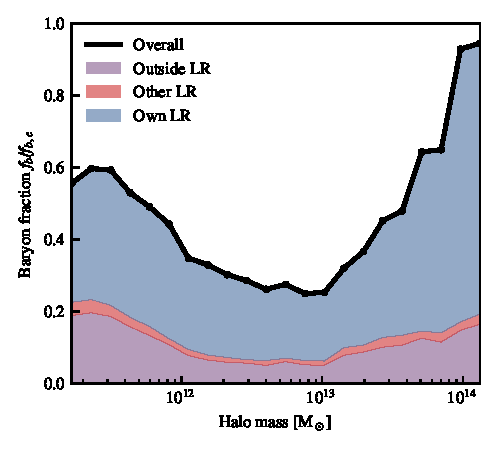
\includegraphics{figures/s50j7kAHF/baryon_fraction_breakdown.pdf}
	\vspace{-0.7cm}
	\caption{The baryon fraction $f_b$ relative to the cosmic baryon fraction
	$f_{b, c}$ shown as a function of halo mass. The coloured bands show the
	contributions to the baryon fraction from various Lagrangian components.}
	\label{fig:baryonfraction}
\end{figure}
\section{Variations on numerical parameters}
\label{sec:convergence}

The above halo-based metrics will have a certain level of dependence on the
choice of halo finder used. In an attempt to ensure independence of the
results from such factors, the above analysis was repeated both with the 3D
friends-of-friends (FoF) halo finder included in the {\tt yt} package
\citep{Turk2011}. We also repeated the analysis with the \velociraptor{} 6D
FoF finder \citep{Elahi2019}. The latter will disentangle active mergers, but
as active mergers make up a small fraction of the galaxy population, the
above results are qualitatively unaffected and only change quantitatively
to the 5\% level. The use of a FoF finder, rather than the spherical
overdensity finder found in AHF, did not qualitatively change the results.

In the below, we discuss ways to extend the Lagrangian region definition to include
more particles, whilst still retaining the ability to have non-uniform shapes. We
find that, in general, including more particles in the definition of the Lagrangian
region (than are present in the halo) leads to a fractionally higher level
of inter-Lagrangian transfer and more self-contribution to the final halo mass
at the expense of transfer from outside any Lagrangian region. This is expected, as
now many more particles are classified as being present in the Lagrangian region.


\subsection{Filling in Holes in Lagrangian Regions}

Our method for producing Lagrangian regions simply uses the dark matter
particles from a given halo; this naturally leads to a very diffuse
Lagrangian region. To see how the diffuse nature of these regions affects our
results, we smooth out the Lagrangian regions, by extending the procedure
that was used to extend the regions from the dark matter to the gas. This
works as follows:
\begin{enumerate}
	\item For every dark matter particle not in a Lagrangian region 
	      in the initial conditions, find the nearest $n$ neighbours.
	\item Find among the neighbours the maximal Lagrangian region ID,
	      corresponding to the lowest mass $z=0$ halo.
	\item Assign the particle the same Lagrangian region ID.
\end{enumerate}
The choice to assign the particles to the lowest mass halo, rather than the
higher mass halo, was made to ensure that spurious transfer into the lower mass
halo was avoided wherever possible. This means that the expectation is that
with this metric the level of inter-Lagrangian transfer will increase with
respect to the fiducial Lagrangian region identification method. The results
with the particles given to the haloes of a higher mass show negligible
deviation from the fiducial result.

\begin{figure}
	\centering
	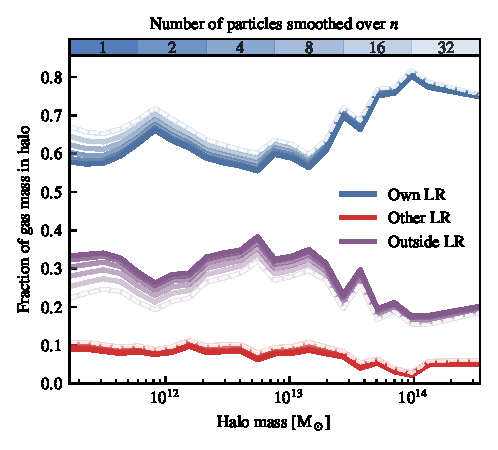
\includegraphics{figures/convergence_smoothing.pdf}
	\vspace{-0.7cm}
 \caption{The same as Fig. \ref{fig:maintransferresult}, but including
 Lagrangian region smoothing. Each line, coded by transparency, shows the
 fraction of baryonic mass in a halo from each component when the Lagrangian
 regions have been smoothed by 1 (i.e. the fiducial result), 2, 4, 8, 16, or
 32 particles (from darkest to lightest respectively). The white dashed line
 shows the result for the 32-smoothing case where the particles are given to
 the highest, rather than lowest, mass haloes; no difference is seen here
 suggesting that there is little overlap between the Lagrangian regions on
 these scales. See the text for the details of how this smoothing is
 constructed.}
	\label{fig:smoothconv}
\end{figure}

The results are shown in Fig. \ref{fig:smoothconv}. Note how smoothing the
Lagrangian regions does have the expected effect of inducing more internal
transfer, and does increase the proportion of baryons that are classified as
retained as the Lagrangian regions are filled out. Despite this, the overall
trends with respect to halo mass remain.

\subsection{The sizes of Lagrangian regions}

In Fig. \ref{fig:bigtransferpic} we saw that there was a large amount of
gaseous matter inside haloes from outside any Lagrangian region. It may be
reasonable to assume that this gas corresponds to dark matter that is simply
sitting just outside of the halo edge, perhaps within the so-called
`splashback radius'. The estimates for this radius range between 0.8 and
1.5$R_{\rm vir}$ \citep{More2015, Diemer2017a}, and hence below we consider
the situation where we extend the region around the halo that contributes to
the Lagrangian region. This is done in the following way:
\begin{enumerate}
	\item For every halo, find its current virial radius $R_{\rm vir}$. This contains
	      all particles at redshift $z=0$ that we consider to be within the halo.
      \item Now consider, $R_{\rm LR}$, and find all dark matter particles within
            this region from the halo centre. These dark matter particles are now
            defined to lie within the Lagrangian region of that halo.
	\item ID match these particles and extend to the gas in the usual way.
\end{enumerate}
We chose this specific process, increasing the radius of our Lagrangian
region rather than the whole halo, to prevent us from simply re-defining our
halo size and including more gas as well (as in this case, the transfer
across the halo boundary would simply be moved to a larger radius). The
effects of this process on the gas component of Fig.
\ref{fig:maintransferresult} (where it is most significant) are shown in Fig.
\ref{fig:radius_dependence}.

\begin{figure}
    \centering
    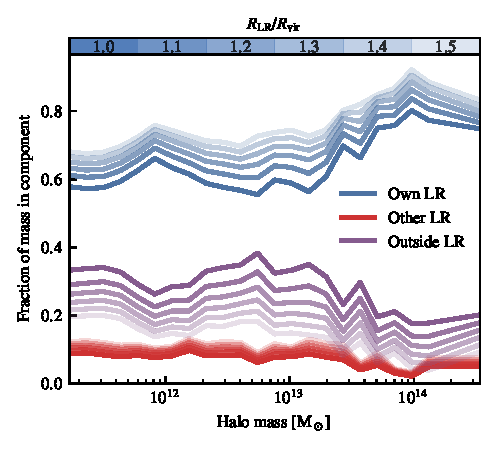
\includegraphics{figures/radius_convergence.pdf}
    \vspace{-0.7cm}
    \caption{Again, the same as Fig. \ref{fig:maintransferresult}, but now
    showing how the Lagrangian make-up of haloes is changed with an increasing
    radius for the Lagrangian region. Lighter colours correspond to larger
    radii, going in steps of $0.1R_{\rm vir}$ from 1.0 to 1.5.}
    \label{fig:radius_dependence}
\end{figure}

Here we see that there is a significant change in the fraction of mass in the
halo at redshift $z=0$ from outside any Lagrangian region, especially when going to
$R_{\rm LR} = 1.5 R_{\rm vir}$. This large change is expected, though, as we now
have included a volume that is three times larger than the initial halo in the
Lagrangian region classification; taking this extreme value for all haloes
really is a `worst-case' scenario. The inter-Lagrangian transfer remains at a similar level
despite the increase in radius. Note that there will be no extra mass included in the
haloes here, with particles simply changing their Lagrangian allegiances.
\section{Discussion}
\label{sec:conclusions}

In the above, we have developed two novel metrics that describe the different
ways in which dark matter and baryons flow in cosmological simulations. The
first, a simple distance metric, shows that it is not just the energetics of
the universe that are changed by the inclusion of AGN jets and other energetic
feedback mechanisms, but that the gas dynamics are changed completely. Whilst
different feedback models may be able to capture the same halo-level metrics
like the galaxy stellar mass function, they necessarily produce vastly
different dynamics. The second, which looks at transfer between lagrangian
regions as defined by the $z=0$ halo population, shows that $5-10\%$ of the
baryonic mass of given halo will have originated from the lagrangian region
of another halo. A common critique of \citet{AnglesAlcazar2017} is that the
majority of the objects that show transfer will have merged by $z=0$. Here,
for the first time, we showed that late-time transfer between halos occurs
in cosmological simulations.

We have also quantified the significant mis-match between the origins of
baryonic and dark matter in halos in cosmological simulations. $40\%$ of the
baryonic mass originates from a different spatial region in the initial
conditions to the dark matter contained in the halo.

We have shown that different lagrangian components, as they make up the
baryon fraction of halos, are affected differently by different feedback
mechanisms. Transfer from outside of any lagrangian region is predominantly
affected by (preventative) AGN feedback in the \simba{} model, whereas gas
that originated in the lagrangian region remains `locked-in' and only a small
proportion is evacuated by feedback.

The transfer between halos has been shown to be a late-time effect, with
there being a negligeable proportion of the $z=2$ baryonic mass of halos
made up of particles from lagrangian regions defined by other halos.

A particularly concerning aspect to the baryon transfer results is that they
have the potential to have huge impacts on semi-analytic models of galaxy
formation. These models, by construction, tie the baryonic matter to dark
matter halos; they contain no prescription for gas that explicitly originates
from regions where the dark matter does not end the simulation in a bound
object. Also, whilst there has been some effort by \citet{Henriques2015} and
others to include wind recycling into these models, there is currently
no semi-analytic model that includes any concept of baryon transfer between
un-merged halos. The mixed origins of the baryons in the $z=0$ halos
point to a different physical origin for many fundamental galaxy properties.


\section{Acknowledgements}
\label{sec:acknowledgements}

The authors would like to thank James Willis for his help with the
\velociraptor{} halo finder, and Aaron Ludlow, Cedric Lacey, Richard Bower,
Shy Genel, Greg Bryan, and Rob Crain for helpful discussions that contributed
significantly to this work.

This work was initiated as a project for the Kavli Summer Program in
Astrophysics held at the Center for Computational Astrophysics of the
Flatiron Institute in 2018. The program was co-funded by the Kavli Foundation
and the Simons Foundation. We thank them for their generous support.

This work was supported by collaborative visits funded by the Cosmology and
Astroparticle Student and Postdoc Exchange Network (CASPEN).

JB is supported by STFC studentship ST/R504725/1. DAA is supported by the
Flatiron Institute, which is supported by the Simons Foundation. This work
used the ARCHER UK National Supercomputing Service.

This work used the DiRAC@Durham facility managed by the Institute for
Computational Cosmology on behalf of the STFC DiRAC HPC Facility
(www.dirac.ac.uk). The equipment was funded by BEIS capital funding via STFC
capital grants ST/K00042X/1, ST/P002293/1, ST/R002371/1 and ST/S002502/1,
Durham University and STFC operations grant ST/R000832/1. DiRAC is part of
the National e-Infrastructure. We would like to extend our thanks specifically
to Alastair Basden and his team for managing the DiRAC Memory Intensive service. 

\subsection{Software Citations}

This paper made use of the following software packages:
\begin{itemize}
    \item GIZMO \citep{Hopkins2017}
        \begin{itemize}
            \item Gadget \citep{Springel2005b}
        \end{itemize}
    \item {\sc Swift} \citep{Schaller2016}
    \item {\tt python} \citep{Rossum1995}, with the following libraries
    \begin{itemize}
    	\item {\tt numpy} \citep{Numpy2006}
    	\item {\tt scipy} \citep{Scipy2001}
    	\item {\tt py-sphviewer} \citep{Benitez-Llambay2015}
    	\item {\tt caesar} \citep{Thompson2018}
    	\item {\tt yt} \citep{Turk2011}
    \end{itemize}
    \item \velociraptor{} \citep{Elahi2019}
    \item The Amiga Halo Finder (AHF) \citep{Gill2004, Knollmann2009}
\end{itemize}




\bibliographystyle{mnras}
\bibliography{bibliography}

\end{document}
